\documentclass[journal]{IEEEtran}
\usepackage{cite}
\usepackage{amsmath,amssymb}
\usepackage{graphicx}
\usepackage{booktabs}
\usepackage{multirow}
\usepackage{xcolor}
\usepackage[hidelinks]{hyperref}
\graphicspath{{../figures/}}
\newcommand{\eg}{e.g.,\ }
\newcommand{\ie}{i.e.,\ }

\begin{document}

\title{Few-Shot, Label-Free Fabric Defect Inspection for Networked Seaming Stations via Confidence-Gated Edge Offloading}

\author{Nasiba Palvannazirova, Ayaz Waseem, Nikita Lobasevich, Petr Butovskiy, and Miralam Allamov%
  \thanks{N. Palvannazirova and A. Waseem are with Electronic Science and Technology, Beijing University of Posts and Telecommunications, Beijing, China (e-mail: nasiba@bupt.edu.cn; 2024090002@bupt.cn).}%
  \thanks{N. Lobasevich is with the School of Economics and Management, Beijing University of Posts and Telecommunications, Beijing, China (e-mail: lnikbest@gmail.com).}%
  \thanks{P. Butovskiy and M. Allamov are with Technological Machines and Apparatus, Tashkent Institute of Textile and Light Industry, Tashkent, Uzbekistan (e-mail: gtnz1071980@gmail.com; miralam3843678@gmail.com).}%
  \thanks{Corresponding author: Petr Butovskiy.}%
  \thanks{Code, configuration, and raw results: [repository URL].}%
}

\markboth{IEEE Internet of Things Journal}{Palvannazirova \MakeLowercase{\textit{et al.}}: Few-Shot, Label-Free Fabric Defect Inspection}

\maketitle

%% ABSTRACT %%

\begin{IEEEkeywords}
Industrial Internet of Things (IIoT), edge computing, computation offloading, MQTT, anomaly detection, fabric defect detection, few-shot learning.
\end{IEEEkeywords}

\section{Introduction}
\IEEEPARstart{F}{abric} inspection is one of the most labour-intensive steps of textile manufacturing. Human inspectors are slow, tire quickly, and miss a substantial fraction of defects, which has motivated two decades of research on automated visual inspection~\cite{kumar2008survey,carrilho2024survey}. The state of the art is dominated by supervised deep detectors and segmenters---improved two-stage detectors~\cite{wu2020cascaded}, efficient single-stage detectors~\cite{zhou2021edds,zhang2022mobilenet}, YOLO-family models on edge hardware~\cite{machado2025textile,nasim2024realworld}, transformer segmenters with Gabor priors~\cite{xu2023swin}, and open-world formulations~\cite{ye2026owdln}. These models reach high accuracy on the fabrics they were trained on, but they require hundreds to thousands of labelled defect instances per fabric family and a GPU-centred training workflow; the scarcity of labelled defects and the cost of retraining for new materials are repeatedly identified as the main obstacles to deployment~\cite{carrilho2024survey}.

The obstacle is acute on the \emph{shop floor of small and medium-sized garment and technical-textile plants}, where a number of seaming or joining machines process short runs of many different fabrics. Our motivating installation is a set of ultrasonic seaming stations, each controlled by an ESP32 micro-controller and an Android application (FabricScope) and equipped with a USB camera that already identifies the fibre and weave before the seam parameters are chosen. A fabric typically stays on a machine for minutes, defects are rare, and there is neither time nor expertise to label data or retrain a model whenever the material changes. Such a deployment is naturally an Industrial Internet of Things (IIoT) system~\cite{sisinni2018iiot}: many low-cost camera nodes, a shared plant network, and at most one modest edge server. The inspection function must therefore (i) learn a new fabric from a few seconds of defect-free material, (ii) set its own decision threshold without defect examples, (iii) run within the frame budget of an inexpensive station node, and (iv) scale to many stations without saturating the uplink or the edge server.

Unsupervised anomaly detection, which learns only from normal samples, satisfies (i) and is an active direction for fabrics~\cite{zhang2026dmglad,ma2025pnemfd,an2025causality}; on generic benchmarks, training-free methods that reuse ImageNet features~\cite{rippel2021gaussian,defard2021padim,roth2022patchcore} are particularly strong. However, these works report threshold-free metrics with hundreds of training images on a GPU, and are silent on (ii)--(iv). Conversely, edge-intelligence research~\cite{shi2016edge,zhou2019edgeintel,li2020edgeai} and fog-based manufacturing inspection~\cite{li2018fog} study where to run inference, but assume supervised models trained offline. To our knowledge, no prior work addresses few-shot, label-free surface inspection \emph{as a networked IIoT service}.

This paper fills that gap with \emph{FabricInspect-IoT}, an open-source three-tier system (station node, edge server, profile registry over MQTT) and an empirical study of its design. Our contributions are:
\begin{enumerate}
\item A \textbf{few-shot, label-free inspection service} in which a fabric is learned from $k$ defect-free frames and two complementary models are built at once: a 5--6\,kB Gabor--colour Gaussian model that runs on the station, and a ResNet-18 nearest-neighbour model (PatchCore-lite) that runs on the edge. Decision thresholds are derived by leave-one-out (LOO) scoring of the $k$ shots, without any defect example.
\item \textbf{Confidence-gated offloading}: the station decides clear cases locally and offloads only frames whose local score falls in an uncertainty band around its LOO threshold. Because both thresholds are label-free, the gate needs no tuning data.
\item A \textbf{profile-distribution mechanism} based on retained MQTT messages, which makes a newly learned fabric available to every station within milliseconds, and an analytical model of uplink load and edge utilisation that predicts how many stations an edge server can support.
\item A \textbf{reproducible evaluation} on the MVTec~AD textures~\cite{bergmann2019mvtec,bergmann2021mvtec} covering few-shot accuracy ($k=1\ldots$all), label-free thresholding, and robustness, together with a live testbed with a production MQTT broker~\cite{light2017mosquitto} and a trace-driven simulator validated against it, which scales the system to 64 stations on emulated Wi-Fi and constrained uplinks and reports end-to-end latency, deadline misses, uplink traffic, and edge utilisation.
\end{enumerate}

The remainder of the paper is organised as follows. Section~\ref{sec:related} reviews related work. Section~\ref{sec:system} presents the architecture and protocol, and Section~\ref{sec:methods} the detectors, the thresholds, the gate, and the load model. Section~\ref{sec:setup} describes the experimental setup, Section~\ref{sec:results} reports the results, and Section~\ref{sec:discussion} discusses limitations before Section~\ref{sec:conclusion} concludes.

\section{Related Work}\label{sec:related}

\subsection{Fabric Defect Detection}
Classical approaches characterise fabric texture with statistical, spectral, and model-based descriptors~\cite{kumar2008survey}. Gabor filters are a recurring choice because their joint spatial--frequency localisation matches the periodic structure of woven and knitted fabric; filter banks~\cite{kumar2002gabor} and optimised filters~\cite{bodnarova2002optimal} separate flaws from regular texture without defect data, and Gabor priors are still used to stabilise modern networks~\cite{xu2023swin}. Supervised deep detectors dominate recent work: cascaded feature pyramids~\cite{wu2020cascaded}, efficient detectors with L-shaped pyramids~\cite{zhou2021edds}, metaheuristic-tuned networks~\cite{alruwais2023moth}, fine-grained space--depth compensation~\cite{zhou2025spacedepth}, and dual-image transformers for periodic lace~\cite{jiao2025lace}. Deployment-oriented studies report MobileNetV2-SSDLite on Jetson Nano with cloud model updates~\cite{zhang2022mobilenet}, YOLOv8 on a real factory data set~\cite{nasim2024realworld}, and YOLOv11 on Jetson Orin with MQTT reporting~\cite{machado2025textile}; all require labelled defects for every product family.

\subsection{Unsupervised and Few-Shot Anomaly Detection}
Learning only from defect-free material avoids labelling. For fabrics, DMGLAD combines teacher--student distillation with global--local reasoning~\cite{zhang2026dmglad}, PNEMFD synthesises feature-level anomalies~\cite{ma2025pnemfd}, UMDNet transfers unbiased knowledge from natural images~\cite{an2025causality}, and OW-DLN incrementally learns unknown defect classes~\cite{ye2026owdln}. These methods train networks for hours on hundreds of images. Training-free alternatives reuse ImageNet features~\cite{he2016resnet}: a single multivariate Gaussian of deep features~\cite{rippel2021gaussian}, per-position Gaussians (PaDiM)~\cite{defard2021padim}, and nearest-neighbour patch memories (PatchCore)~\cite{roth2022patchcore}. They are fitted in seconds, which makes them candidates for per-fabric learning at the machine, but their behaviour with very few shots, without labelled thresholds, and on CPUs has not been characterised for textiles.

\subsection{Edge Intelligence and Offloading in the IIoT}
Edge computing moves computation close to data sources to reduce latency and backhaul traffic~\cite{shi2016edge,mao2017mec}. For deep inference, the main design levers are partitioning a network between device and server (Neurosurgeon~\cite{kang2017neurosurgeon}, Edgent~\cite{li2020edgeai}), early exits that stop computation once confidence is sufficient (BranchyNet~\cite{teerapittayanon2016branchynet}), and fog-assisted inspection pipelines in factories~\cite{li2018fog}; Zhou \textit{et al.}~\cite{zhou2019edgeintel} survey the field. These approaches assume a supervised model whose confidence is calibrated on labelled data. Our gate is in the spirit of early exiting, but between two \emph{different} label-free models on two tiers, with the exit band derived from LOO statistics of normal shots only. MQTT~\cite{mqtt311} is the de-facto publish/subscribe protocol in IIoT; we use its retained messages to distribute fabric models.

\subsection{Material Identification at the Machine}
Beyond surface defects, sorting and processing lines identify fibre composition, \eg by near-infrared spectroscopy~\cite{cura2021nir,li2025fabricnet}, and X-ray scattering reveals internal fibre shifts in fabric-reinforced composites~\cite{ozturk2023xray}. In our installation the station already classifies the material to set ultrasonic seam parameters; FabricInspect-IoT adds the missing surface-quality check in front of the seam, reusing the same camera.

\section{System Architecture}\label{sec:system}

\begin{figure}[t]
\centering
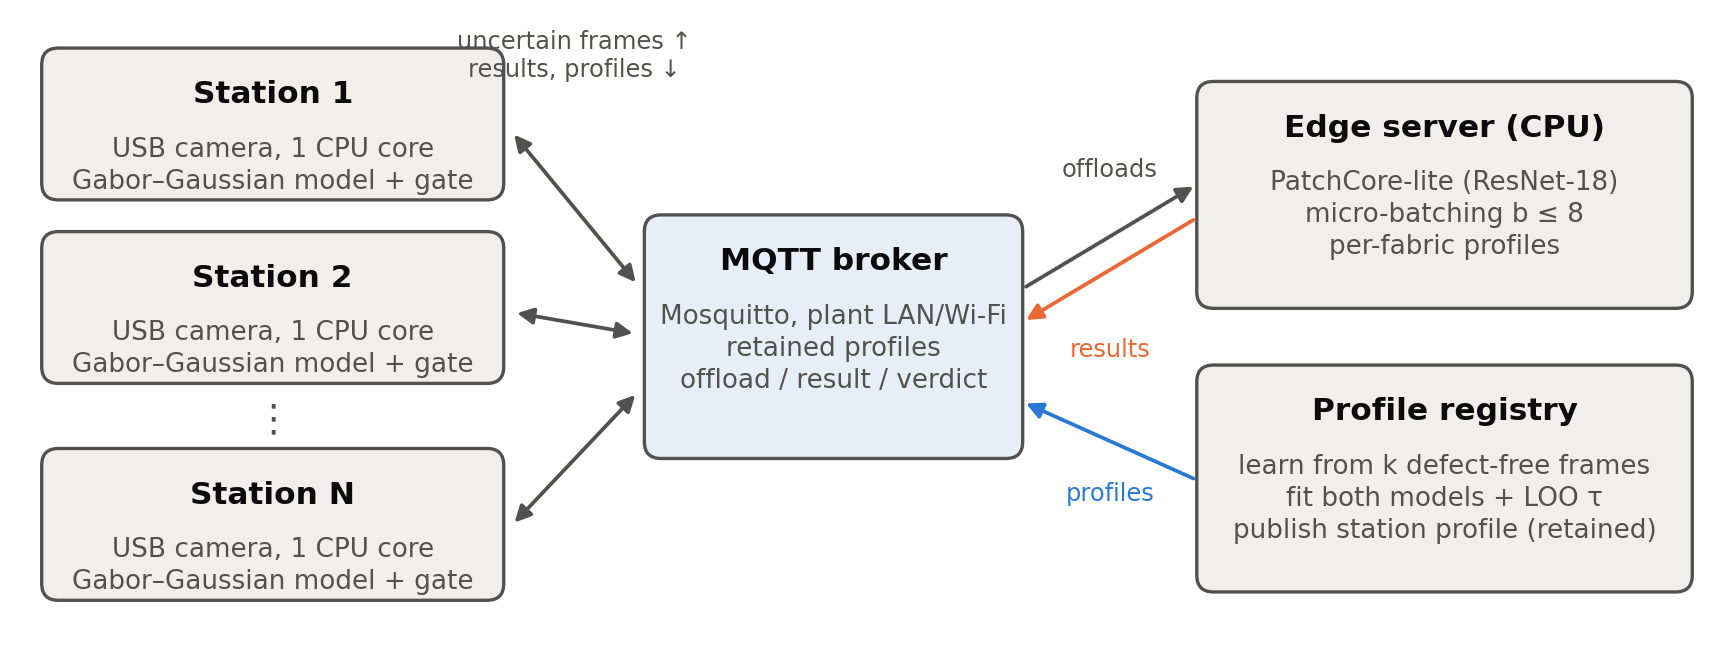
\includegraphics[width=\columnwidth]{fig_architecture.png}
\caption{FabricInspect-IoT. The registry learns a fabric once from $k$ defect-free frames, publishes the compact station model as a retained MQTT message, and installs the deep model on the edge. Stations score every frame and offload only uncertain ones.}
\label{fig:arch}
\end{figure}

Fig.~\ref{fig:arch} shows the three tiers. \emph{Station node:} each seaming machine carries a USB camera looking at the fabric in front of the seam line and a small computer (in our installation the machine's Android controller; in the experiments one CPU core). It holds only the station profile of the current fabric, scores each frame with the Gabor--Gaussian detector (Section~\ref{sec:gg}), and applies the confidence gate (Section~\ref{sec:gate}). \emph{Edge server:} one plant-level x86 machine without GPU subscribes to the offloaded frames of all stations, groups pending requests into micro-batches of up to $b_{\max}=8$, scores them with the PatchCore-lite model of the corresponding fabric (Section~\ref{sec:pc}), and returns the result. \emph{Profile registry:} when an operator learns a new fabric, the registry fits both models from the same $k$ frames, computes both thresholds, publishes the station profile as a \emph{retained} MQTT message, and stores the edge profile on the server. Because the broker keeps the last retained message per topic, a station that starts, reboots, or switches to that fabric receives the model immediately on subscription.

All communication uses MQTT~3.1.1~\cite{mqtt311} through a standard broker (Mosquitto~\cite{light2017mosquitto}) on four topics: \texttt{fi/profile/<fabric>/gabor} (station model, QoS~1, retained), \texttt{fi/st/<id>/offload} (JSON header plus $256\times256$ JPEG crop at quality 85, QoS~1), \texttt{fi/st/<id>/result} (JSON score and verdict, QoS~1), and \texttt{fi/st/<id>/verdict} (informational, QoS~0).

In \emph{learn} mode the operator slowly moves defect-free material under the camera while a frame is grabbed every 0.4\,s until $k$ frames (default 10) are collected. In \emph{inspect} mode each frame is centre-cropped, scored, and shown with a heat-map whose above-threshold regions are outlined; every decision is logged and defective frames are saved for review. A desktop GUI, a command-line interface, and the three IoT roles share one detector module, so the numbers in this paper are produced by the code an operator runs. The implementation uses Python, OpenCV, SciPy, Eclipse Paho, and PyTorch (CPU) with public ImageNet ResNet-18 weights~\cite{he2016resnet}.

\section{Detection, Thresholding, and Offloading}\label{sec:methods}

All detectors receive a colour image resized to $256\times256$ pixels, are fitted on $k$ defect-free images only, and return an anomaly map $A(\mathbf{x})$ that is bilinearly up-sampled from the feature grid and smoothed with a Gaussian ($\sigma=4$\,px). The image score is $s=\max_{\mathbf{x}}A(\mathbf{x})$.

\subsection{Station Model: Gabor--Gaussian}\label{sec:gg}
The image is converted to CIE L*a*b*. The lightness channel $L$ is filtered with quadrature Gabor pairs at wavelengths $\lambda\in\{4,8,16\}$\,px and orientations $\theta\in\{0^\circ,45^\circ,90^\circ,135^\circ\}$ (envelope $\sigma=0.56\lambda$, aspect ratio 0.5), giving 12 energy maps
\begin{equation}
E_{\lambda,\theta}=\sqrt{\left(L\star g^{\mathrm{e}}_{\lambda,\theta}\right)^2+\left(L\star g^{\mathrm{o}}_{\lambda,\theta}\right)^2}.
\end{equation}
All 24 correlations are computed with one FFT of the reflect-padded image and 12 inverse FFTs of precomputed complex spectra, which is numerically equivalent to spatial filtering (max.\ relative deviation $<10^{-6}$) but about $3\times$ cheaper on one core. For the 12 energies and for $L$, $a^*$, $b^*$, local mean and standard deviation over a $15\times15$ window are sampled with stride 4, yielding a $D=30$-dimensional descriptor $\mathbf{f}(\mathbf{x})$ on a $64\times64$ grid. Because fabric texture is approximately stationary, a \emph{single} Gaussian $\mathcal{N}(\boldsymbol{\mu},\boldsymbol{\Sigma})$ is fitted to the descriptors of all positions of all shots (at most $2\cdot10^5$ randomly chosen vectors), with ridge regularisation $\boldsymbol{\Sigma}_\epsilon=\boldsymbol{\Sigma}+\epsilon\,(\operatorname{tr}\boldsymbol{\Sigma}/D)\,\mathbf{I}$, $\epsilon=0.01$, and
\begin{equation}
A(\mathbf{x})=\sqrt{(\mathbf{f}(\mathbf{x})-\boldsymbol{\mu})^{\top}\boldsymbol{\Sigma}_\epsilon^{-1}(\mathbf{f}(\mathbf{x})-\boldsymbol{\mu})}.
\end{equation}
Sharing one Gaussian across positions means that even a single image supplies 4096 training vectors, so the model is usable at $k=1$. The profile consists of $D+D^2=930$ numbers plus the threshold.

\subsection{Edge Model: PatchCore-lite}\label{sec:pc}
Following PatchCore~\cite{roth2022patchcore}, ResNet-18 layer-2 ($128\times32\times32$) and layer-3 ($256\times16\times16$) features are averaged over $3\times3$ neighbourhoods, layer~3 is up-sampled to $32\times32$, and the two are concatenated into 384-dimensional patch descriptors. All descriptors of the $k$ shots form a memory bank that is randomly subsampled to 10\,\% (at least 1000 entries); a test patch is scored by its Euclidean distance to the nearest bank entry. Random rather than greedy-coreset subsampling keeps fitting essentially instantaneous; we therefore call the method PatchCore-lite. As a third, position-specific reference we also evaluate PaDiM~\cite{defard2021padim} (ResNet-18 layers 1--3, 100 random channels, one Gaussian per position), which is not deployed because its per-position statistics make the profile large and LOO calibration expensive.

\subsection{Label-Free Thresholds by Leave-One-Out}\label{sec:loo}
When a new fabric is learned, no defect examples exist. For each shot $i$ the detector is refitted on the other $k-1$ shots and the score $s_i^{\mathrm{LOO}}$ of shot $i$ is computed; these scores estimate the score distribution of \emph{unseen} defect-free frames (scoring the training shots with the full model would be biased low---for a nearest-neighbour model, trivially zero). The threshold is
\begin{equation}
\tau=(1+m)\max_{i=1..k}s_i^{\mathrm{LOO}},\label{eq:tau}
\end{equation}
with margin $m=0.1$ by default. LOO costs $k$ refits on cached features: milliseconds for the Gabor--Gaussian model and well under a second for PatchCore-lite at $k=10$. We denote the station and edge thresholds by $\tau_g$ and $\tau_p$.

\subsection{Confidence-Gated Offloading}\label{sec:gate}
Let $s_g$ be the station score of a frame. With $0<\alpha\le1\le\beta$, the station
\begin{equation}
\text{decision}=\begin{cases}
\text{OK (local)}, & s_g<\alpha\,\tau_g,\\
\text{DEFECT (local)}, & s_g>\beta\,\tau_g,\\
\text{offload}\;\Rightarrow\;\text{DEFECT iff } s_p>\tau_p, & \text{otherwise},
\end{cases}\label{eq:gate}
\end{equation}
where $s_p$ is the edge score. $\alpha=\beta=1$ reduces to station-only inspection; $\alpha\to0,\beta\to\infty$ to edge-only. Both thresholds come from (\ref{eq:tau}), so the band is expressed in units of the fabric's own normal-score scale and transfers across fabrics without labelled tuning. We fix $\alpha=0.6,\beta=1.5$ a priori and report the full $(\alpha,\beta)$ trade-off in Section~\ref{sec:res-gate}.

\subsection{Load Model}\label{sec:load}
Let $N$ stations capture $f$ frames/s, a fraction $o$ of which are offloaded with mean payload $J$ bytes (plus MQTT/TCP/IP overhead $h$). The per-station uplink rate and the edge utilisation are
\begin{equation}
R_{\mathrm{up}}=8fo(J+h),\qquad \rho=\frac{Nfo}{\mu(b)},\label{eq:load}
\end{equation}
where $\mu(b)$ is the edge throughput (frames/s) at batch size $b$. The edge can serve at most $N_{\max}=\mu/(fo)$ stations; cutting $o$ by gating raises $N_{\max}$ proportionally. The end-to-end latency of an offloaded frame is approximately
\begin{equation}
T\approx t_g+\frac{8(J+h)}{B}+2d+W_q+t_p(b),\label{eq:latency}
\end{equation}
with station compute $t_g$, uplink bit-rate $B$, one-way delay $d$, queueing delay $W_q$, and edge compute $t_p$; locally decided frames take $t_g$ only. Section~\ref{sec:res-live} compares (\ref{eq:load}) with measurements.

\section{Experimental Setup}\label{sec:setup}

\subsection{Data}
Openly downloadable, pixel-annotated fabric-defect benchmarks are scarce; the AITEX database~\cite{silvestre2019aitex} could not be obtained without registration at the time of writing. We therefore use the five texture categories of MVTec~AD~\cite{bergmann2019mvtec,bergmann2021mvtec}---carpet, grid, leather, tile, and wood---as stationary-texture proxies for the materials processed on joining machines: carpet is a woven textile, grid a regular mesh, leather a sheet material seamed on the same class of machines, and tile and wood test generality. Each category provides 230--280 defect-free training images and 78--124 test images with pixel masks covering five defect types (\eg cut, hole, thread, colour, metal contamination, fold, crack). The data set is released under CC BY-NC-SA~4.0.

\subsection{Protocol and Metrics}
For each category, $k$ defect-free images are drawn at random from the training split, $k\in\{1,2,5,10,20,50,\text{all}\}$, with three random draws (one for ``all''). Test images are never used for fitting, thresholding or gating. Threshold-free detection is measured by image-level AUROC; localisation by pixel-level AUROC and by AUPRO up to 30\,\% false-positive rate~\cite{bergmann2021mvtec}. With the label-free thresholds we report the false-alarm rate on good images (FPR), defect recall, precision, and F1. The Gabor--Gaussian descriptor (wavelengths, window, colour statistics) was fixed in a preliminary exploration on the same categories at $k=20$; to make this visible we report the complete ablation (Section~\ref{sec:res-ablation}). The gate band $(\alpha,\beta)=(0.6,1.5)$ was fixed before the gate experiments were run.

\subsection{Live Deployment}
The live experiments run the actual system: Eclipse Mosquitto~2.1.2 as broker, one edge server process (8 PyTorch threads, micro-batch $b_{\max}=8$), and $N\in\{1,4,8,16,32\}$ station processes, each restricted to one CPU thread. Station $i$ inspects the test images of category $i \bmod 5$ in random order at $f=5$ frames/s, a rate that covers a $\approx$50\,mm field of view at seam speeds up to $\approx$15\,m/min without gaps. Each station is fitted with $k=10$ shots. Uplinks are emulated at the application layer (Fig.~\ref{fig:arch}): every station owns a FIFO link with bit-rate $B$ and one-way delay $d$---``Wi-Fi'' ($B=20$\,Mbit/s, $d=4$\,ms) and ``constrained'' ($B=1$\,Mbit/s, $d=40$\,ms)---and incoming results are delayed by $d$. A decision is counted as a deadline miss if it is not available at the station within one frame period (200\,ms). Three policies are compared: station-only ($\alpha=\beta=1$), edge-only (thin station, every frame offloaded), and the gated cascade.

\subsection{Hardware and Software}
All processes run on one host (Intel Core i9-14900HX, 24 cores/32 threads, 32\,GB RAM, Windows~11) with Python~3.9, PyTorch~2.8 (CPU), OpenCV~5.0, SciPy~1.13, and Paho-MQTT~2.1; no GPU is used. Restricting stations to one thread approximates a low-cost single-board station node; edge and stations share the host, which is conservative for the edge (Section~\ref{sec:discussion}).

\section{Results}\label{sec:results}

\subsection{Few-Shot Detection}\label{sec:res-fewshot}
Table~\ref{tab:k10} lists all metrics at the default $k=10$; the complete curves for $k=1\ldots$all are in the repository. \emph{PatchCore-lite is the most accurate detector at every $k$}: averaged over the five textures its image AUROC is 0.904 with a single shot, 0.916 at $k=10$, and 0.977 with the full training set (AUPRO 0.747, 0.786, 0.894). \emph{The stationary Gabor--Gaussian model is the most shot-efficient}: it reaches 0.828 at $k=1$---better than PaDiM (0.725), whose per-position Gaussians are poorly estimated from few images---and saturates early (0.860 at $k=10$, 0.872 with all shots). The gap between station and edge model is \emph{fabric-dependent}: on leather, tile, and wood the station model is within 0.07 AUROC of PatchCore-lite, whereas on carpet (0.740 vs.\ 0.967) and grid (0.674 vs.\ 0.636) it is not adequate at $k=10$. Grid is hard for all detectors with few shots and improves with more normal data (PatchCore-lite 0.921 with all 264 images).

Fig.~\ref{fig:qual} shows typical anomaly maps. Both models localise the carpet thread, the leather cut, and the tile crack, and both miss the small broken cells of the grid. On wood the colour-sensitive station model flags the bleached scratch whereas PatchCore-lite stays below its threshold: the models are complementary rather than nested. This fabric dependence motivates the two-tier design.

\begin{table*}[t]
\centering
\caption{Detection and localisation with $k=10$ defect-free shots (mean of three random draws). GG: Gabor--Gaussian (station), PC: PatchCore-lite (edge), PD: PaDiM. Best per metric in bold.}
\label{tab:k10}
\footnotesize
\begin{tabular}{@{}lccccccccc@{}}
\toprule
& \multicolumn{3}{c}{Image AUROC} & \multicolumn{3}{c}{Pixel AUROC} & \multicolumn{3}{c}{AUPRO} \\
\cmidrule(lr){2-4}\cmidrule(lr){5-7}\cmidrule(l){8-10}
Category & GG & PC & PD & GG & PC & PD & GG & PC & PD \\
\midrule
carpet & 0.740 & \textbf{0.967} & 0.881 & 0.883 & \textbf{0.988} & 0.972 & 0.643 & \textbf{0.933} & 0.911 \\
grid & \textbf{0.674} & 0.636 & 0.633 & 0.621 & \textbf{0.742} & 0.676 & 0.178 & \textbf{0.333} & 0.330 \\
leather & 0.984 & \textbf{0.999} & 0.961 & \textbf{0.993} & 0.992 & 0.989 & \textbf{0.984} & 0.965 & 0.967 \\
tile & 0.919 & \textbf{0.986} & 0.841 & 0.936 & \textbf{0.940} & 0.820 & 0.768 & \textbf{0.817} & 0.606 \\
wood & 0.981 & \textbf{0.992} & 0.989 & \textbf{0.932} & 0.929 & 0.931 & 0.879 & 0.882 & \textbf{0.908} \\ \midrule
\textit{Mean} & 0.860 & \textbf{0.916} & 0.861 & 0.873 & \textbf{0.918} & 0.878 & 0.690 & \textbf{0.786} & 0.744 \\
\bottomrule
\end{tabular}
\end{table*}


\begin{figure}[t]
\centering
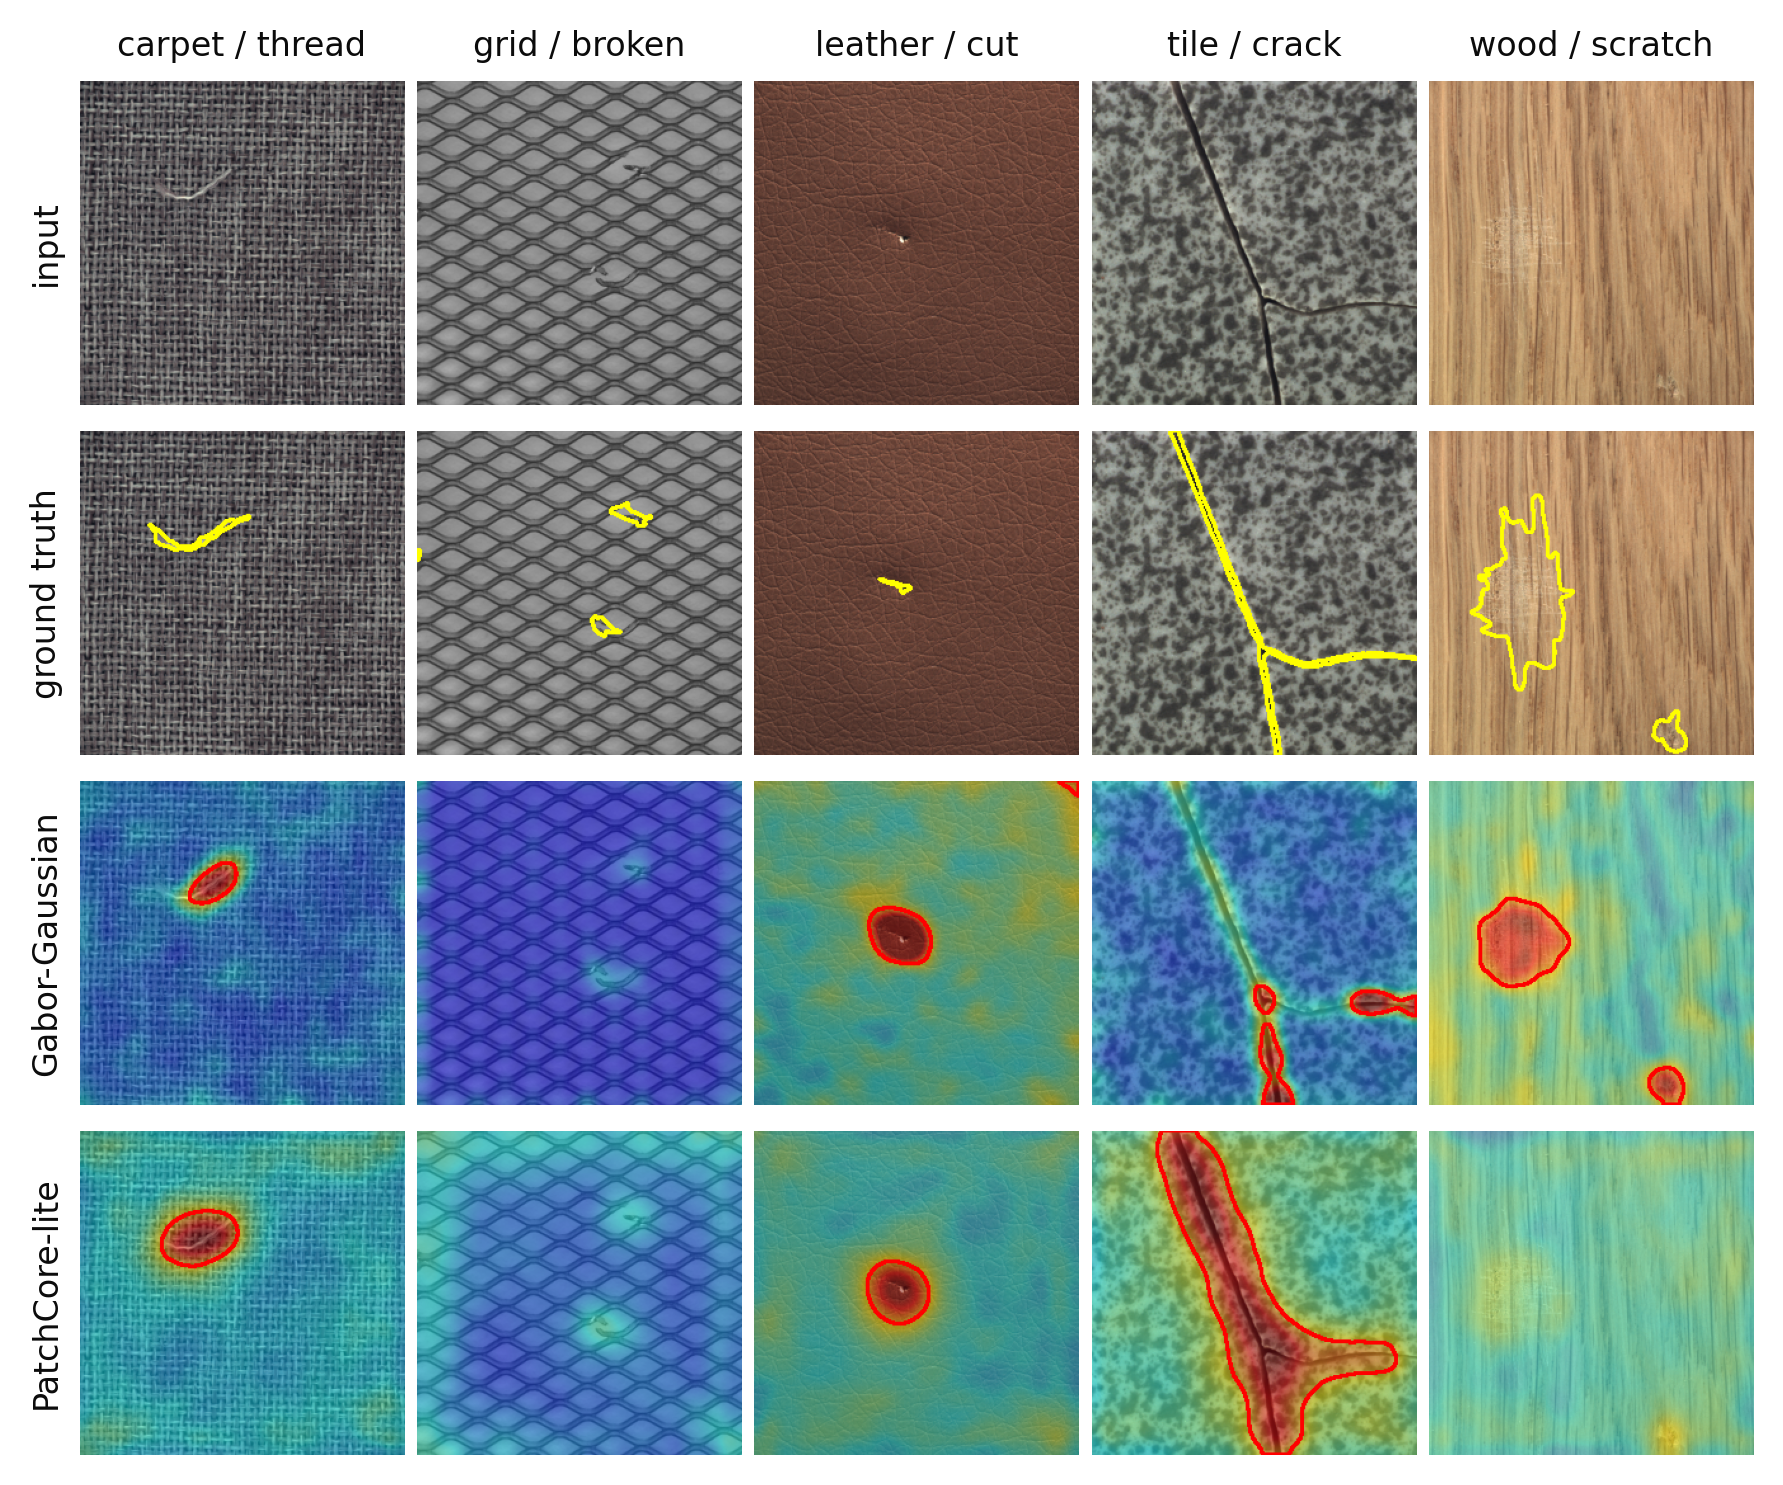
\includegraphics[width=\columnwidth]{fig_qualitative.png}
\caption{Anomaly maps of the station (Gabor--Gaussian) and edge (PatchCore-lite) models ($k=10$). Yellow: ground truth; red: regions above the label-free threshold.}
\label{fig:qual}
\end{figure}

\subsection{Label-Free Thresholds}\label{sec:res-threshold}
With the LOO threshold (\ref{eq:tau}), PatchCore-lite at $k=10$ and $m=0.1$ produces 3.4\,\% false alarms on good test images at 71.8\,\% defect recall (F1 0.753, mean of five textures and three draws). Without margin, recall rises to 78.8\,\% but false alarms to 24.5\,\%; $m=0.2$ removes false alarms entirely at 65.3\,\% recall, so $m$ is a single, interpretable knob between nuisance stops and escapes. Results are similar for $k=5$ and $20$ (F1 0.755 and 0.754). Grid is the exception: its LOO threshold is so conservative that almost no defect is flagged (F1 0.023); on the other four textures PatchCore-lite reaches F1 0.935 at 4.3\,\% false alarms and 89.4\,\% recall. The station model's LOO threshold is far less reliable (28.2\,\% false alarms at $k=10$, $m=0.1$), dominated by leather (95.8\,\%) and carpet (38.1\,\%), where ten LOO scores underestimate the range of normal scores. The station threshold is therefore best used to \emph{define} an uncertainty band rather than to issue final verdicts near the boundary.

\begin{table*}[t]
\centering
\caption{Detection and localisation with $k=10$ defect-free shots (mean of three random draws). GG: Gabor--Gaussian (station), PC: PatchCore-lite (edge), PD: PaDiM. Best per metric in bold.}
\label{tab:k10}
\footnotesize
\begin{tabular}{@{}lccccccccc@{}}
\toprule
& \multicolumn{3}{c}{Image AUROC} & \multicolumn{3}{c}{Pixel AUROC} & \multicolumn{3}{c}{AUPRO} \\
\cmidrule(lr){2-4}\cmidrule(lr){5-7}\cmidrule(l){8-10}
Category & GG & PC & PD & GG & PC & PD & GG & PC & PD \\
\midrule
carpet & 0.740 & \textbf{0.967} & 0.881 & 0.883 & \textbf{0.988} & 0.972 & 0.643 & \textbf{0.933} & 0.911 \\
grid & \textbf{0.674} & 0.636 & 0.633 & 0.621 & \textbf{0.742} & 0.676 & 0.178 & \textbf{0.333} & 0.330 \\
leather & 0.984 & \textbf{0.999} & 0.961 & \textbf{0.993} & 0.992 & 0.989 & \textbf{0.984} & 0.965 & 0.967 \\
tile & 0.919 & \textbf{0.986} & 0.841 & 0.936 & \textbf{0.940} & 0.820 & 0.768 & \textbf{0.817} & 0.606 \\
wood & 0.981 & \textbf{0.992} & 0.989 & \textbf{0.932} & 0.929 & 0.931 & 0.879 & 0.882 & \textbf{0.908} \\ \midrule
\textit{Mean} & 0.860 & \textbf{0.916} & 0.861 & 0.873 & \textbf{0.918} & 0.878 & 0.690 & \textbf{0.786} & 0.744 \\
\bottomrule
\end{tabular}
\end{table*}

\begin{table}[t]
\centering
\caption{Decisions with the label-free LOO threshold (\ref{eq:tau}); mean over five categories and three draws. FPR: false alarms on good test images.}
\label{tab:threshold}
\footnotesize
\begin{tabular}{@{}lcccccc@{}}
\toprule
Model & $k$ & $m$ & FPR & Recall & Prec. & F1 \\
\midrule
GG (station) & 10 & 0.0 & 0.335 & 0.670 & 0.901 & 0.693 \\
 & 10 & 0.1 & 0.282 & 0.624 & 0.777 & 0.659 \\
 & 10 & 0.2 & 0.225 & 0.577 & 0.797 & 0.624 \\
 & 10 & 0.3 & 0.180 & 0.541 & 0.814 & 0.593 \\
 & 5 & 0.1 & 0.176 & 0.569 & 0.816 & 0.617 \\
 & 20 & 0.1 & 0.206 & 0.602 & 0.800 & 0.645 \\ \midrule
PC (edge) & 10 & 0.0 & 0.245 & 0.788 & 0.851 & 0.778 \\
 & 10 & 0.1 & 0.034 & 0.718 & 0.855 & 0.753 \\
 & 10 & 0.2 & 0.000 & 0.653 & 0.800 & 0.713 \\
 & 10 & 0.3 & 0.000 & 0.573 & 0.800 & 0.653 \\
 & 5 & 0.1 & 0.071 & 0.734 & 0.812 & 0.755 \\
 & 20 & 0.1 & 0.025 & 0.722 & 0.858 & 0.754 \\
\bottomrule
\end{tabular}
\end{table}

Grid is the exception in Table~\ref{tab:threshold}: its LOO threshold is so conservative that almost no defect is flagged (recall 1.2\,\%, F1 0.023 for PatchCore-lite), which lowers every five-category mean. On the other four textures PatchCore-lite with $k=10$, $m=0.1$ reaches F1 0.935 at 4.3\,\% FPR and 89.4\,\% recall.

\subsection{Confidence-Gated Offloading}\label{sec:res-gate}
Fig.~\ref{fig:gate} shows the accuracy--offload trade-off obtained by sweeping $\alpha\in[0.3,1]$ for three values of $\beta$, and Table~\ref{tab:gate} details the a-priori operating point. Station-only inspection never offloads but reaches only F1 0.659 with 28.2\,\% false alarms; edge-only inspection reaches F1 0.753 at 3.4\,\% FPR but offloads every frame. The gated cascade with $(\alpha,\beta)=(0.6,1.5)$ attains F1 0.748---99.3\,\% of the edge-only value---while offloading 50.9\,\% of frames, and cuts the station-only false-alarm rate from 28.2\,\% to 7.9\,\%. Excluding grid, the cascade reaches F1 0.930 versus 0.935 for edge-only and 0.801 for station-only. Along the Pareto front, $(\alpha,\beta)=(0.7,1.5)$ keeps F1 at 0.739 with 39.8\,\% offload, and $(0.6,2.0)$ matches edge-only (0.753) with 61.8\,\%; the lower bound of the band, $\alpha$, controls how many frames are trusted as clearly normal and is the dominant knob, whereas $\beta=\infty$ (never declaring defects locally) wastes offloads on frames the station already recognises as defective.

The gate adapts to the fabric automatically (Table~\ref{tab:gate}): it offloads only 23\,\% of leather and 30\,\% of wood frames, where the station model is already strong, but 81\,\% of carpet frames, where it is weak. This is the desired behaviour of an uncertainty-driven policy, and it emerges from the LOO thresholds alone, without any labelled tuning per fabric. It also corrects the station's worst failure, the 95.8\,\% false-alarm rate on leather, to 19.8\,\%. The residual gap to edge-only on leather (FPR 4.2\,\%) comes from frames whose station score exceeds $\beta\tau_g$ although they are defect-free, which a larger $\beta$ removes at the cost of more offloads.

\begin{figure}[t]
\centering
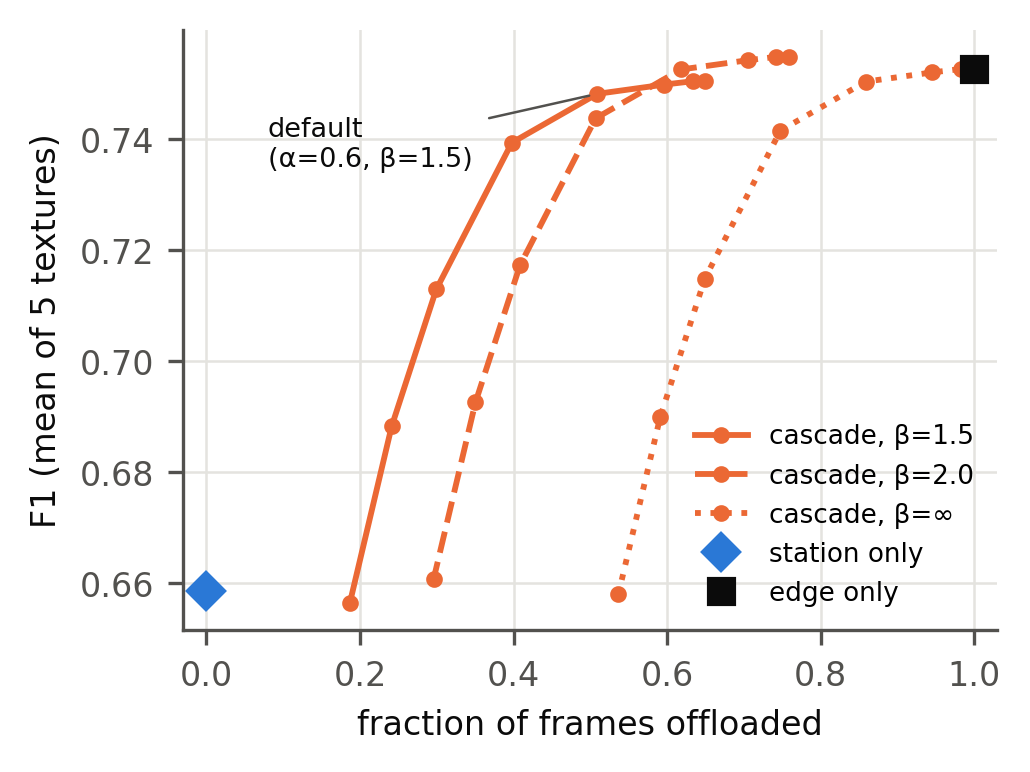
\includegraphics[width=\columnwidth]{fig_gate.png}
\caption{Accuracy--offload trade-off of the gate ($k=10$, mean of five textures and three draws). Each curve sweeps $\alpha$ from 1.0 (left) to 0.3 (right).}
\label{fig:gate}
\end{figure}

\begin{table}[t]
\centering
\caption{Per-fabric decisions of the three policies ($k=10$, $m=0.1$, mean of three draws). Cascade uses the a-priori band $\alpha=0.6,\beta=1.5$; ``off.'' is the offloaded fraction.}
\label{tab:gate}
\footnotesize
\setlength{\tabcolsep}{3.5pt}
\begin{tabular}{@{}lccccccc@{}}
\toprule
& \multicolumn{2}{c}{Station only} & \multicolumn{3}{c}{Cascade} & \multicolumn{2}{c}{Edge only} \\
\cmidrule(lr){2-3}\cmidrule(lr){4-6}\cmidrule(l){7-8}
Category & F1 & FPR & F1 & FPR & off. & F1 & FPR \\
\midrule
carpet & 0.718 & 0.381 & 0.918 & 0.143 & 0.81 & 0.923 & 0.095 \\
grid & 0.090 & 0.016 & 0.023 & 0.000 & 0.52 & 0.023 & 0.000 \\
leather & 0.857 & 0.958 & 0.963 & 0.198 & 0.23 & 0.985 & 0.042 \\
tile & 0.717 & 0.000 & 0.880 & 0.000 & 0.68 & 0.872 & 0.000 \\
wood & 0.911 & 0.053 & 0.957 & 0.053 & 0.30 & 0.960 & 0.035 \\ \midrule
\textit{Mean} & 0.659 & 0.282 & 0.748 & 0.079 & 0.51 & 0.753 & 0.034 \\
\bottomrule
\end{tabular}
\end{table}


\subsection{Resources, Profiles, Ablation, and Robustness}\label{sec:res-resources}
On one core the station model needs 36.1\,ms per frame (p95 40.3\,ms), \ie it sustains 27 frames/s, more than five times the inspection rate, without any deep-learning runtime. Its serialised profile is 5.0--6.1\,kB, whereas a PatchCore-lite memory bank occupies 1.1--1.3\,MB and a PaDiM model 165\,MB, which rules PaDiM out for distribution. With eight threads the edge model scores a frame in 16--20\,ms including JPEG decoding; micro-batching raises its throughput $\mu$ from 64 frames/s at $b=1$ to 96 frames/s at $b=8$. Learning a fabric from $k=10$ frames, including both LOO calibrations, takes 0.55--0.96\,s for the station model and 0.17\,s for PatchCore-lite. The retained station profile reaches every subscribed station in 10--15\,ms on the Wi-Fi link and 93\,ms on the constrained link, independently of whether 1, 8, or 32 stations subscribe; a PatchCore-lite profile would need 0.52\,s and 10.1\,s. A fabric change thus costs seconds of operator time, not a deployment step.

\emph{Ablation} ($k=20$): removing the Lab chroma statistics from the station descriptor costs 0.029 image AUROC and 0.065 AUPRO, since colour defects are invisible to a greyscale texture model; removing the Gabor bank costs 0.039 and 0.108. Six orientations instead of four add 0.016 AUROC at 40\,\% more dimensions and filter cost; we keep four as a compromise between accuracy, compute, and profile size.

\emph{Robustness} ($k=20$, test frames perturbed at working resolution, models fitted on clean shots): $\pm$20\,\% brightness changes AUROC by at most 0.009 for all detectors, since a global gain shifts good and defective scores alike. Defocus blur ($\sigma=2$\,px) costs 0.08--0.12 for all detectors. Sensor noise ($\sigma=10$ grey levels) affects the station model most ($-0.128$, its finest Gabor scale responds to pixel noise) and PatchCore-lite least ($-0.048$). A change of focus, lighting, or camera should therefore be followed by re-learning the fabric, which takes seconds and needs no labels.

\subsection{System Performance and Scalability}\label{sec:res-live}

\emph{Methodology.} Hour-long live sweeps with up to 32 station processes, a broker, and an edge server on one laptop proved unsuitable for timing: under sustained load the host repeatedly entered power-limited states in which all code ran 4--8$\times$ slower, and the station processes competed for cores that real stations would not share. We therefore measure the service-time distributions of every component in short, speed-checked runs (station model: 300 frames on one core; edge: 60 batches for each $b=1\ldots8$; JPEG payloads of all test frames) and feed them into a trace-driven discrete-event simulator of Fig.~\ref{fig:arch}: periodic capture, a single-core station, a FIFO uplink per station with the emulated rate and delay, a single batching edge server ($b_{\max}=8$), and the downlink delay. About 15\,\% of the edge samples were 5--10$\times$ slower than the median because of the same host throttling; samples above twice the median are excluded, and a slower edge is studied explicitly below. The only free parameter, a constant messaging and serialisation overhead per offloaded frame, is calibrated on one live configuration (Wi-Fi, edge-only, $N=1$): 38.7\,ms.

\emph{Validation.} Table~\ref{tab:validation} compares the simulator with short live runs of the complete system. On Wi-Fi the simulated median latency of the cascade is within 7\,ms of the live value and its p95 within 28\,ms; for edge-only with $N=4$ the live p95 is 60\,ms higher. Deadline-miss rates agree in every Wi-Fi configuration and, on the constrained link, within 15 percentage points. The live edge was 1.4--2.6$\times$ busier than simulated in the unflagged configurations, because on the testbed it shares the CPU with the station processes and the broker; the ``edge 2$\times$ slower'' scenario brackets this case. Four live runs show signs of transient host throttling (marked $\dagger$).

\begin{table}[t]
\centering
\caption{Validation of the trace-driven simulator against the live testbed (live / simulated, both 12\,s at 5 frames/s; simulation: mean of 20 seeds). Latency in ms, misses in \%. $^\dagger$Live run affected by transient host throttling (station median $>2\times$ its trace median, or edge utilisation $>3\times$ simulated).}
\label{tab:validation}
\footnotesize
\setlength{\tabcolsep}{3pt}
\begin{tabular}{@{}llccccc@{}}
\toprule
Link & Policy & $N$ & p50 & p95 & Miss & Edge util. \\
\midrule
wifi$^\dagger$ & station-only & 1 & 143 / 36 & 161 / 40 & 0.0 / 0.0 & 0.00 / 0.00 \\
wifi & station-only & 4 & 53 / 36 & 75 / 40 & 0.0 / 0.0 & 0.00 / 0.00 \\
wifi & cascade & 1 & 115 / 108 & 143 / 115 & 0.0 / 0.0 & 0.16 / 0.06 \\
wifi & cascade & 4 & 94 / 99 & 142 / 115 & 0.0 / 0.0 & 0.24 / 0.18 \\
wifi & edge-only & 1 & 73 / 73 & 80 / 78 & 0.0 / 0.0 & 0.20 / 0.08 \\
wifi & edge-only & 4 & 96 / 73 & 143 / 83 & 0.0 / 0.0 & 0.55 / 0.32 \\
constrained & station-only & 1 & 46 / 36 & 153 / 40 & 0.0 / 0.0 & 0.00 / 0.00 \\
constrained$^\dagger$ & station-only & 4 & 170 / 36 & 191 / 40 & 0.8 / 0.0 & 0.00 / 0.00 \\
constrained$^\dagger$ & cascade & 1 & 678 / 402 & 807 / 498 & 95.0 / 80.5 & 0.61 / 0.06 \\
constrained$^\dagger$ & cascade & 4 & 679 / 310 & 1482 / 447 & 60.0 / 56.1 & 0.96 / 0.18 \\
constrained & edge-only & 1 & 683 / 667 & 1016 / 953 & 100.0 / 100.0 & 0.15 / 0.07 \\
constrained & edge-only & 4 & 1095 / 290 & 3556 / 855 & 100.0 / 100.0 & 0.80 / 0.31 \\
\bottomrule
\end{tabular}
\end{table}


\begin{figure*}[t]
\centering
\includegraphics[width=0.92\textwidth]{fig_sim.png}
\caption{Validated trace-driven simulation on the Wi-Fi link (10 seeds $\times$ 60\,s per point): p95 decision latency (dashed line: 200-ms frame period), deadline misses, and edge utilisation versus the number of stations. Dotted: edge server twice as slow; thin dashed: load model (\ref{eq:load}) with $\mu(8)$.}
\label{fig:sim}
\end{figure*}

\emph{Scaling on Wi-Fi} (Fig.~\ref{fig:sim}). Station-only inspection scales trivially---each decision takes 40\,ms (p95) on the station's own core and no uplink is used---but inherits the station model's accuracy (F1 0.659). Edge-only inspection meets the 200-ms deadline for up to $N=16$ stations (p95 154\,ms, 0.3\,\% misses), at which point the edge is saturated ($\rho=0.99$); at $N=24$ virtually every decision is late. The cascade supports $N=24$ stations (p95 155\,ms, 0.2\,\% misses, $\rho=0.87$) and degrades gracefully: at $N=32$ only 13.6\,\% of decisions miss the deadline, and even in overload at most the offloaded half is late, because clear cases are still decided locally. With an edge twice as slow, the cascade supports 8 stations and edge-only 4. The cascade thus raises the number of stations per edge server by 1.5--2$\times$ while delivering 99\,\% of the edge-only F1, and reduces the mean uplink per station from 821 to 504\,kbit/s (39\,\%). The load model (\ref{eq:load}) with $\mu(8)=96$ frames/s predicts saturation at $N_{\max}=\mu/(fo)\approx19$ stations for edge-only and $\approx37$ for the cascade ($o=0.52$), consistent with the simulated knees between 16--24 and 24--32 stations; at light load it underestimates utilisation because batches are small ($\mu(1)=64$). It is a useful first-order sizing rule: one CPU edge server per $\approx\!\mu/(fo)$ stations.

\emph{Constrained uplinks.} At 1\,Mbit/s a single 14--26\,kB offload needs 110--210\,ms of transmission, which alone exhausts the 200-ms budget. Edge-only decisions are therefore always late (100\,\% misses for every $N$), the cascade misses essentially its offloaded fraction (51--53\,\% for $N\ge8$), and only station-only inspection meets the deadline. On such links the station model must take all time-critical decisions; offloaded verdicts remain useful as delayed quality records, or the payload must shrink (smaller crop, stronger compression).

\subsection{Profile Distribution}\label{sec:res-profile}
Learning a new fabric from $k=10$ frames, including both LOO calibrations, took 0.55--0.96\,s for the station model and 0.17\,s for PatchCore-lite (3.6\,s on the very first fabric, which includes loading the ResNet-18 weights). Publishing the 6.1\,kB station profile as a retained message delivered it to every subscribed station in 10--15\,ms over the Wi-Fi link and in 93\,ms over the constrained link, independently of whether 1, 8, or 32 stations subscribed, because the broker fans the message out once per station link. Distributing a PatchCore-lite profile instead (1.25\,MB) would take 0.52\,s and 10.1\,s, respectively. A fabric change therefore costs the plant a few seconds of operator time for capturing frames, not a model-deployment step.

\subsection{Robustness to Imaging Conditions}\label{sec:res-robust}
Table~\ref{tab:robust} applies global brightness changes, defocus blur, and sensor noise to the test frames at the $256\times256$ working resolution, with models fitted on clean shots. All detectors are insensitive to $\pm$20\,\% brightness in terms of AUROC (at most $-0.009$): a global gain shifts the scores of good and defective frames alike, so their ranking is preserved, although the absolute LOO threshold may then be off. Blur ($\sigma=2$\,px) costs 0.08--0.12 AUROC for all three detectors because it removes the fine texture that both Gabor energies and early ResNet layers rely on. Noise ($\sigma=10$ grey levels) affects the station model most ($-0.128$), since its finest Gabor scale ($\lambda=4$\,px) responds to pixel noise, and PatchCore-lite least ($-0.048$). In practice, a change of focus, lighting or camera should be followed by re-learning the fabric, which, as shown above, takes seconds and needs no labels; the logged score distribution of recent OK frames can be used to trigger it automatically.

\begin{table*}[t]
\centering
\caption{Robustness of image AUROC to imaging changes applied to the test frames only ($k=20$, mean over five categories; change w.r.t.\ clean in parentheses).}
\label{tab:robust}
\footnotesize
\begin{tabular}{@{}lccccc@{}}
\toprule
Model & none & bright-20\% & bright+20\% & blur($\sigma$=2) & noise($\sigma$=10) \\
\midrule
GG & 0.872 & 0.879 (+0.007) & 0.864 (-0.008) & 0.772 (-0.099) & 0.744 (-0.128) \\
PC & 0.957 & 0.955 (-0.002) & 0.957 (+0.000) & 0.878 (-0.079) & 0.909 (-0.048) \\
PD & 0.904 & 0.895 (-0.009) & 0.903 (-0.001) & 0.783 (-0.121) & 0.850 (-0.054) \\
\bottomrule
\end{tabular}
\end{table*}


\section{Discussion and Limitations}\label{sec:discussion}

\emph{Data.} The evaluation uses MVTec~AD textures as a proxy for fabrics because openly downloadable, pixel-annotated textile data sets are scarce. Carpet and grid are the closest analogues of woven fabric and are also the hardest categories for the station model; leather, tile, and wood are easier. Validation on images captured at the seaming machines themselves---which the system logs automatically, including every flagged frame---is the most important next step.

\emph{Thresholds.} The LOO rule is label-free and works well for the edge model on four of five textures, but it fails on grid, where the normal-score distribution of ten shots does not cover the variability of the test images. More shots help (Section~\ref{sec:res-fewshot}); an operator-in-the-loop update that adds confirmed false alarms to the memory bank is a simple remedy that the logging already supports.

\emph{Emulation.} Stations, broker, and edge server share one host and the links are emulated at the application layer, so radio effects (contention, retransmissions, jitter bursts) are not captured, and the station CPU is a single core of a laptop processor rather than an embedded board. Sharing the host is pessimistic for the edge server, which competes with up to 32 station processes for cores. To ease replication on real hardware, the repository contains a stand-alone station benchmark that needs only NumPy, SciPy, and OpenCV. Energy consumption was not measured.

\emph{Scope.} The system detects anomalies; it does not name the defect type. Classifying flagged frames, for example with a small supervised model trained incrementally on the logged snapshots, would turn the inspection log into a labelled data set over time. Security of the MQTT deployment (TLS, authentication, access control lists) is supported by standard brokers but was disabled in the experiments.

\section{Conclusion}\label{sec:conclusion}
We presented FabricInspect-IoT, a few-shot, label-free fabric inspection service for networked seaming stations, and characterised it as an IIoT system. A fabric is learned from ten defect-free frames in about a second; a 6\,kB station model and a ResNet-18 nearest-neighbour edge model are fitted together, and both obtain their decision thresholds by leave-one-out scoring of the shots, without any defect example. With these thresholds, the edge model reaches F1 0.935 at 4.3\,\% false alarms on four of five MVTec~AD textures, while the fifth (grid) exposes the limits of ten-shot calibration. Confidence-gated offloading retains 99\,\% of the edge-only F1 while sending only half of the frames to the edge and lowers the station-only false-alarm rate from 28\,\% to 8\,\%; the gate adapts its offload rate to the fabric (23--81\,\%) using only the label-free thresholds. In a live deployment with a production MQTT broker, [TBD: live-system summary]. Retained MQTT messages distribute a new fabric model to any number of stations within 15\,ms on Wi-Fi.

Future work will validate the system on images logged at the seaming machines, port the station model to the machines' Android controllers, add operator feedback to refine the LOO thresholds, and extend the gate to adapt $\alpha$ to the instantaneous edge load and uplink quality.

\section*{Author Contributions}
N.~Palvannazirova: conceptualization, methodology, software, investigation, data curation, writing---original draft preparation. A.~Waseem: software, formal analysis, validation, writing---review and editing. N.~Lobasevich: formal analysis, visualization, writing---review and editing. P.~Butovskiy: supervision, methodology, validation, writing---review and editing. M.~Allamov: investigation, resources, validation, writing---review and editing.

\section*{Acknowledgment}
[To be completed by the authors.]

\section*{Use of AI-Assisted Tools}
[To be completed by the authors, following IEEE's policy on AI-generated content: name the tool(s), the sections or code they assisted with, and confirm that the authors reviewed and take responsibility for all content.]


\bibliographystyle{IEEEtran}
\bibliography{refs}

\end{document}
